\appendix
\appendixpage
\addappheadtotoc
%
% \begin{figure}%[H]
%   \begin{center}
%   \includegraphics[width=0.8\textwidth]{}
%   \end{center}
%   \caption{Left panel shows data over the quake location, right panel shows data over the ribbon location. From top to bottom, plots show lightcurves from IRIS Si IV, Mg II, Balmer wavelengths and Mg II wing, with the bottom panel showing the lightcurve from SDO HMI.}\label{lcseries-bold}
% \end{figure}

%insert figure showing ribbon coords oplot
%\graphicspath{ {~/PhD/Thesis/upgrade-plots/}}


%contains energy time plots for quake and ribbon locations
%also contains energy tables


%\includegraphics[trim=left bottom right top, clip]{file}
\begin{figure}[H]
  \begin{center}
  \textbf{Quake Location Energy Over Time}\par\medskip
  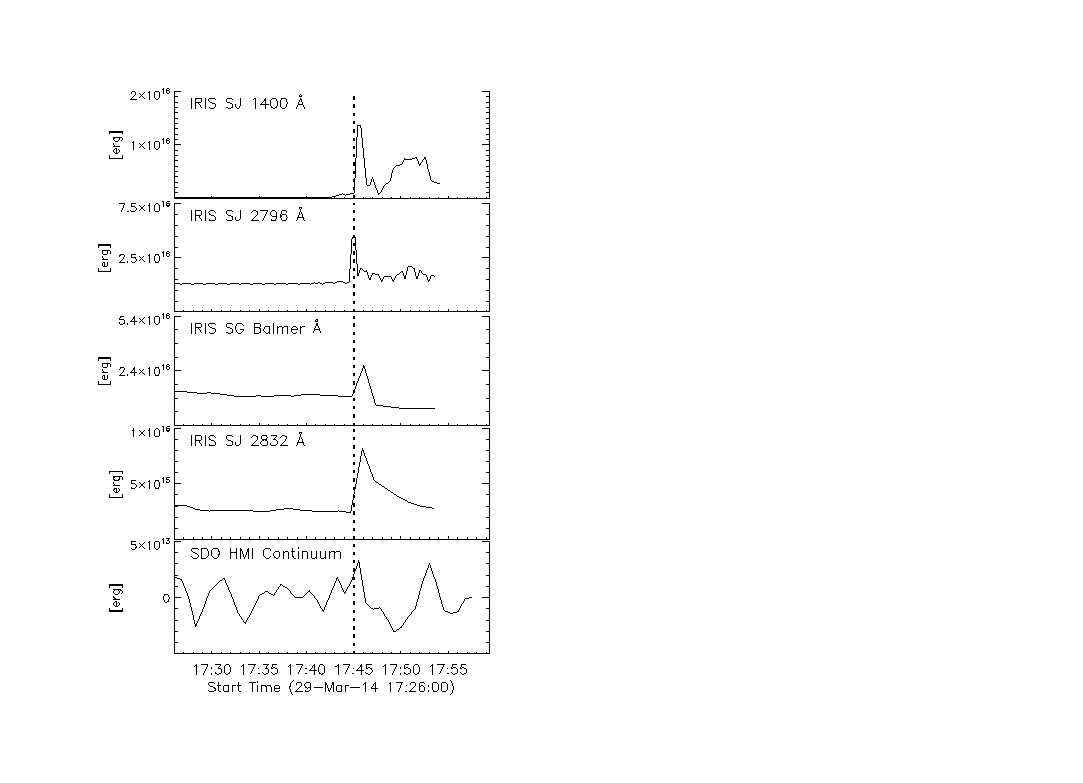
\includegraphics[width=0.6\textwidth]{29-Mar-14-Quake-Energy-Ladder}
  \end{center}
  \caption{Shows calculated energy values over time of the region thought to be the sunquake epicenter (518.5", 264.0"). Each plot represents an independant data set, in order from top to bottom the sets are; IRIS SJ 1400 \AA\ (Si IV); IRIS SJ 2796 \AA\ (Mg II); IRIS SG  2825.7 to 2825.8 \AA\ (Balmer Continuum);IRIS SJ 2832 \AA\ (Mg II wing); SDO HMI continuum (HMI).}\label{eqk}
\end{figure}

\begin{figure}[H]
  \begin{center}
  \textbf{Energy Over Time, Ribbon Location: x = 517, y = 260 }\par\medskip
  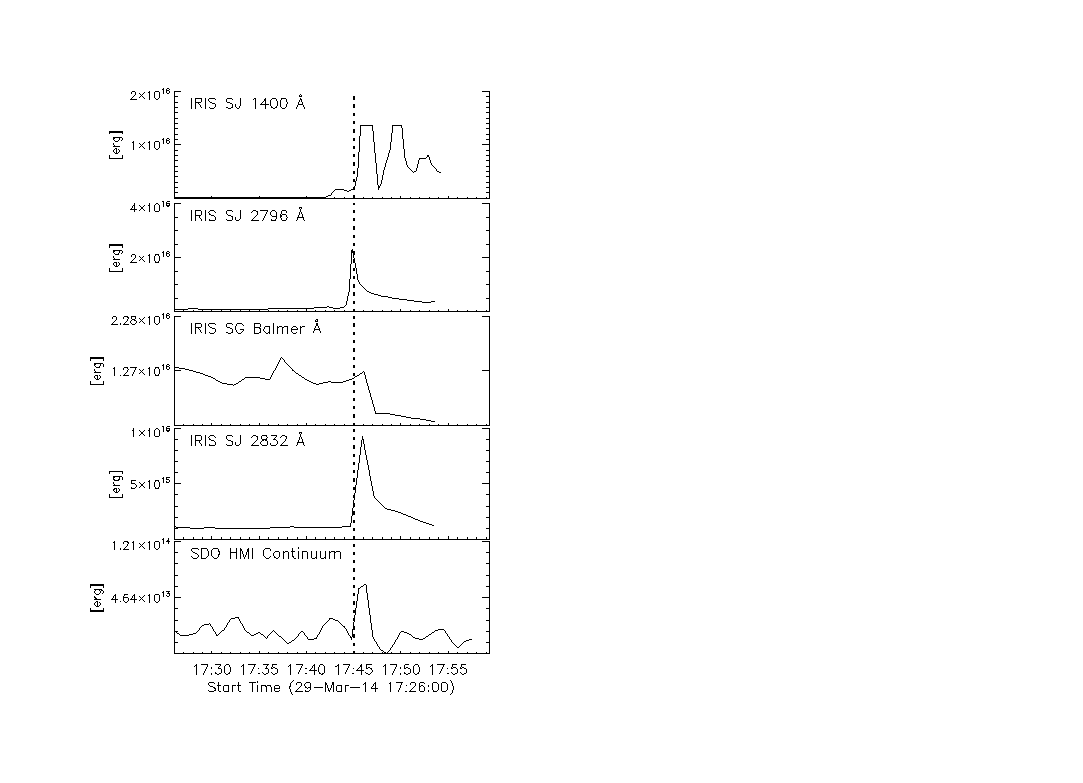
\includegraphics[width=0.6\textwidth]{29-Mar-14-Ribbon-xyPosition-517-260-Frame-1-Energy-Ladder}
  \end{center}
  \caption{Shows calculated energy (erg) values over time (UT) for the heliocentric coordinates (arcsec) contained in the plot title. Each plot represents an independant data set, in order from top to bottom the sets are; IRIS SJ 1400 \AA\ (Si IV); IRIS SJ 2796 \AA\ (Mg II); IRIS SG  2825.7 to 2825.8 \AA\ (Balmer Continuum);IRIS SJ 2832 \AA\ (Mg II wing); SDO HMI continuum (HMI).}\label{erb1}
\end{figure}

\begin{figure}[H]
  \begin{center}
  \textbf{Energy Over Time, Ribbon Location: x = 518, y = 261 }\par\medskip
  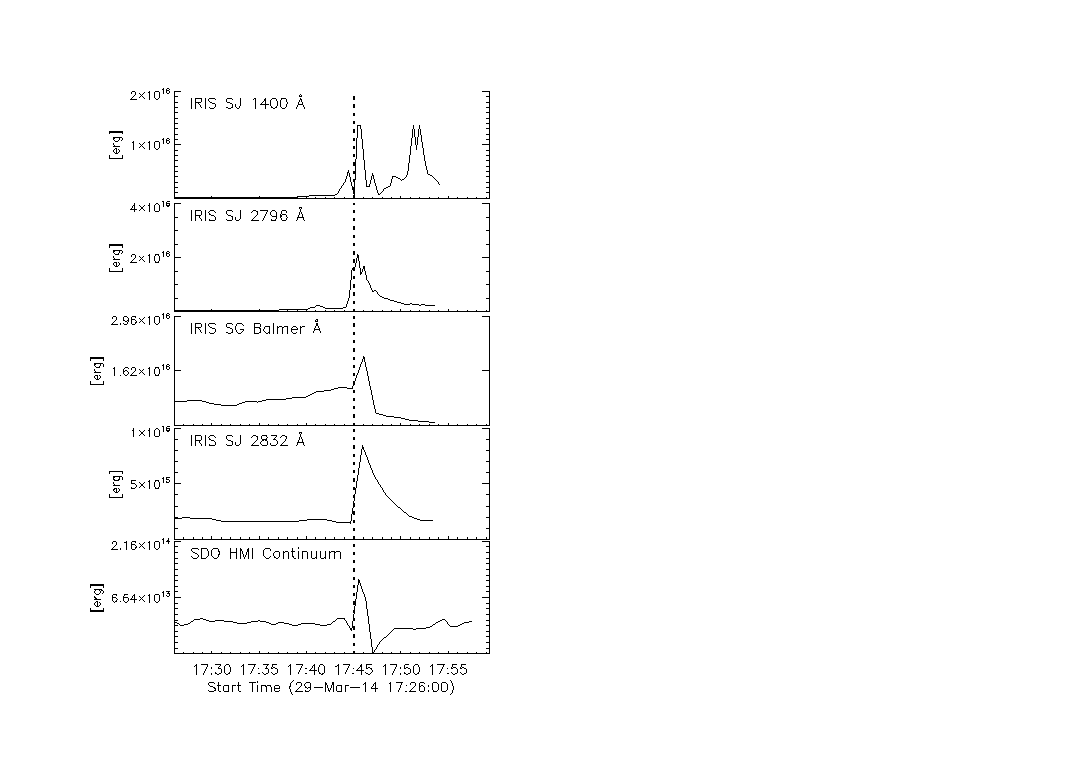
\includegraphics[width=0.6\textwidth]{29-Mar-14-Ribbon-xyPosition-518-261-Frame-1-Energy-Ladder}
  \end{center}
  \caption{Shows calculated energy (erg) values over time (UT) for the heliocentric coordinates (arcsec) contained in the plot title. Each plot represents an independant data set, in order from top to bottom the sets are; IRIS SJ 1400 \AA\ (Si IV); IRIS SJ 2796 \AA\ (Mg II); IRIS SG  2825.7 to 2825.8 \AA\ (Balmer Continuum);IRIS SJ 2832 \AA\ (Mg II wing); SDO HMI continuum (HMI).}\label{erb2}
\end{figure}


\begin{figure}[H]
  \begin{center}
  \textbf{Energy Over Time, Ribbon Location: x = 519, y = 261 }\par\medskip
  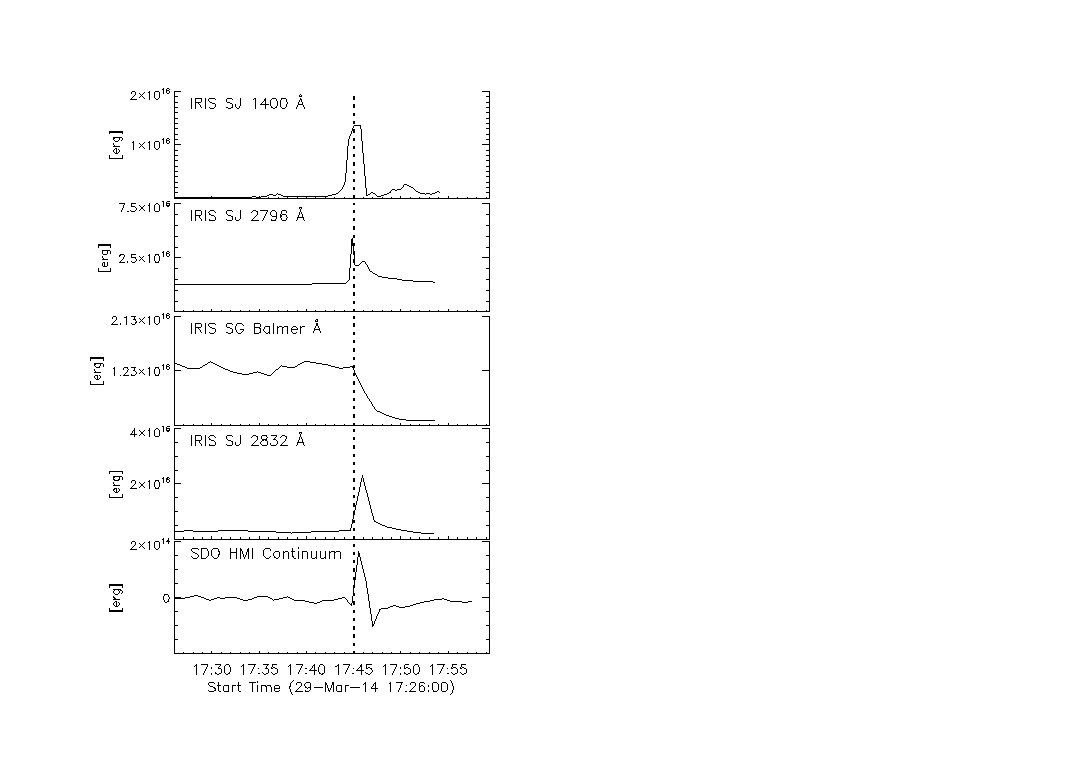
\includegraphics[width=0.6\textwidth]{29-Mar-14-Ribbon-xyPosition-519-261-Frame-1-Energy-Ladder}
  \end{center}
  \caption{Shows calculated energy (erg) values over time (UT) for the heliocentric coordinates (arcsec) contained in the plot title. Each plot represents an independant data set, in order from top to bottom the sets are; IRIS SJ 1400 \AA\ (Si IV); IRIS SJ 2796 \AA\ (Mg II); IRIS SG  2825.7 to 2825.8 \AA\ (Balmer Continuum);IRIS SJ 2832 \AA\ (Mg II wing); SDO HMI continuum (HMI).}\label{erb3}
\end{figure}

\begin{figure}[H]
  \begin{center}
  \textbf{Energy Over Time, Ribbon Location: x = 520, y = 262 }\par\medskip
  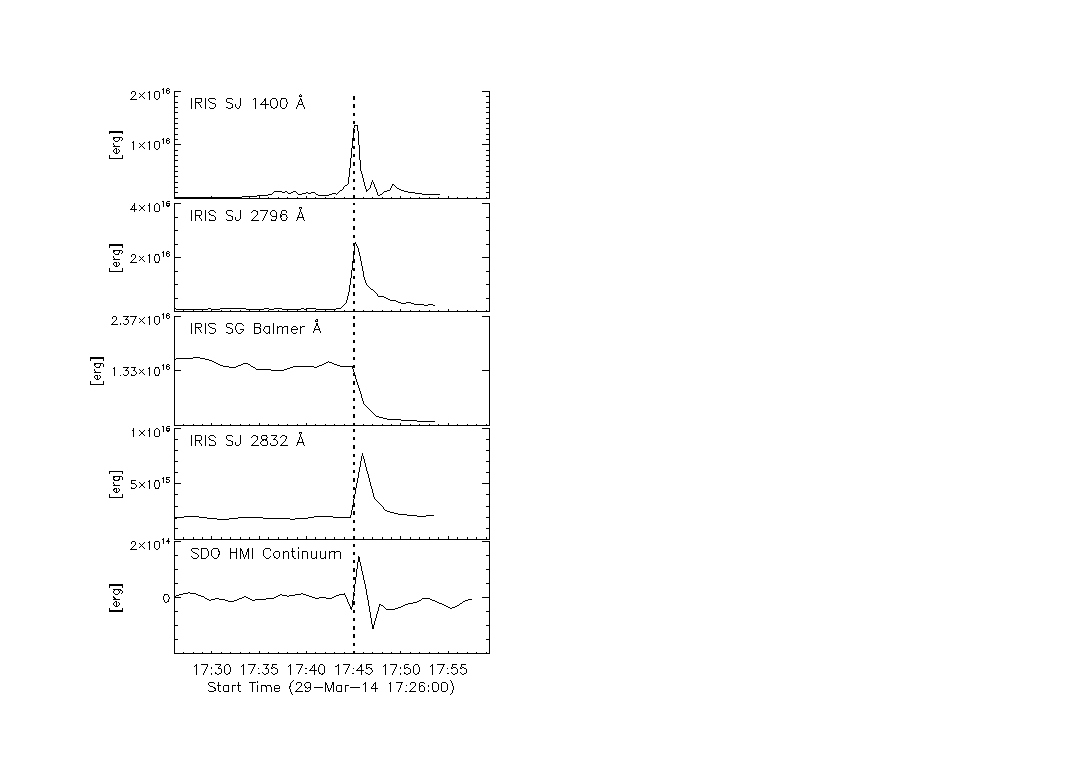
\includegraphics[width=0.6\textwidth]{29-Mar-14-Ribbon-xyPosition-520-262-Frame-1-Energy-Ladder}
  \end{center}
  \caption{Shows calculated energy (erg) values over time (UT) for the heliocentric coordinates (arcsec) contained in the plot title. Each plot represents an independant data set, in order from top to bottom the sets are; IRIS SJ 1400 \AA\ (Si IV); IRIS SJ 2796 \AA\ (Mg II); IRIS SG  2825.7 to 2825.8 \AA\ (Balmer Continuum);IRIS SJ 2832 \AA\ (Mg II wing); SDO HMI continuum (HMI).}\label{erb4}
\end{figure}

\begin{figure}[H]
  \begin{center}
  \textbf{Energy Over Time, Ribbon Location: x = 521, y = 262 }\par\medskip
  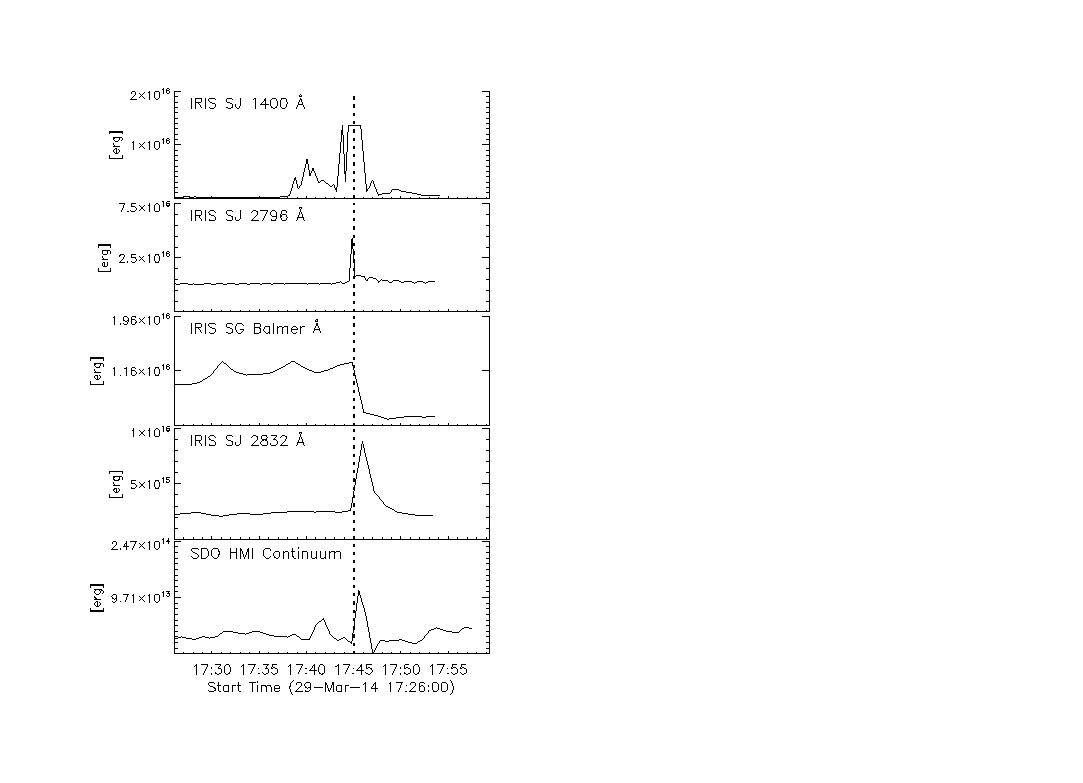
\includegraphics[width=0.6\textwidth]{29-Mar-14-Ribbon-xyPosition-521-262-Frame-1-Energy-Ladder}
  \end{center}
  \caption{Shows calculated energy (erg) values over time (UT) for the heliocentric coordinates (arcsec) contained in the plot title. Each plot represents an independant data set, in order from top to bottom the sets are; IRIS SJ 1400 \AA\ (Si IV); IRIS SJ 2796 \AA\ (Mg II); IRIS SG  2825.7 to 2825.8 \AA\ (Balmer Continuum);IRIS SJ 2832 \AA\ (Mg II wing); SDO HMI continuum (HMI).}\label{erb5}
\end{figure}

\begin{figure}[H]
  \begin{center}
  \textbf{Energy Over Time, Ribbon Location: x = 500, y = 262 }\par\medskip
  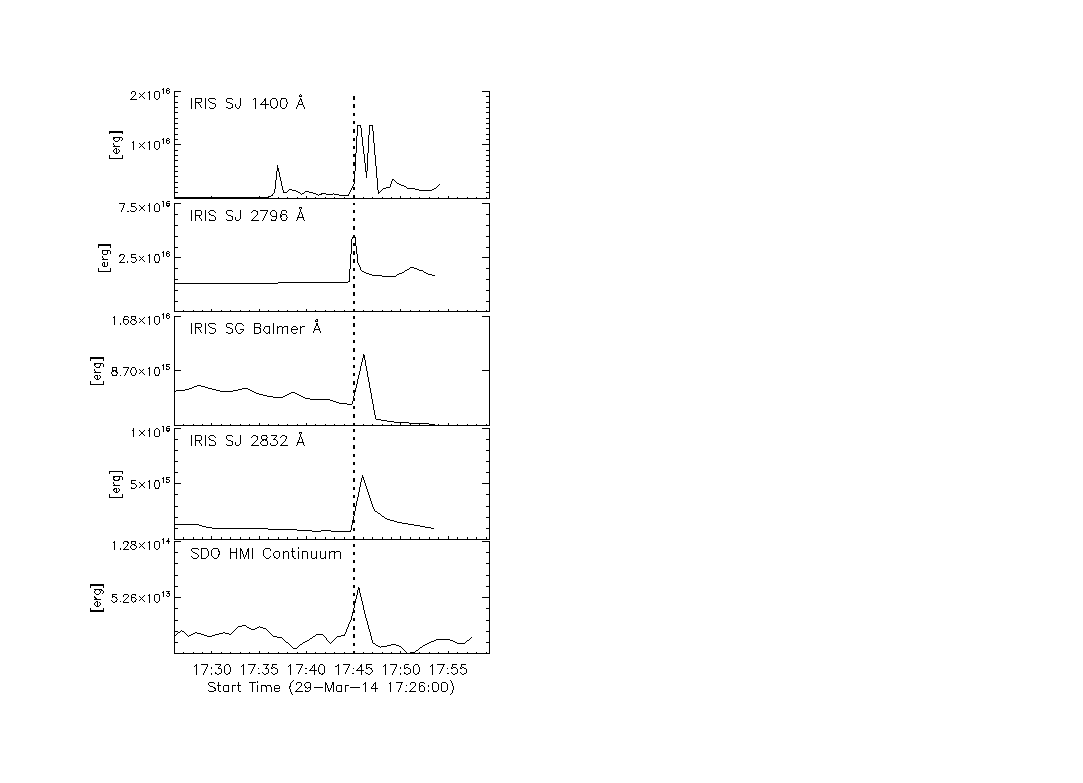
\includegraphics[width=0.6\textwidth]{29-Mar-14-Ribbon-xyPosition-500-262-Frame-1-Energy-Ladder}
  \end{center}
  \caption{Shows calculated energy (erg) values over time (UT) for the heliocentric coordinates (arcsec) contained in the plot title. Each plot represents an independant data set, in order from top to bottom the sets are; IRIS SJ 1400 \AA\ (Si IV); IRIS SJ 2796 \AA\ (Mg II); IRIS SG  2825.7 to 2825.8 \AA\ (Balmer Continuum);IRIS SJ 2832 \AA\ (Mg II wing); SDO HMI continuum (HMI).}\label{erb6}
\end{figure}

\begin{figure}[H]
  \begin{center}
  \textbf{Energy Over Time, Ribbon Location: x = 503, y = 265 }\par\medskip
  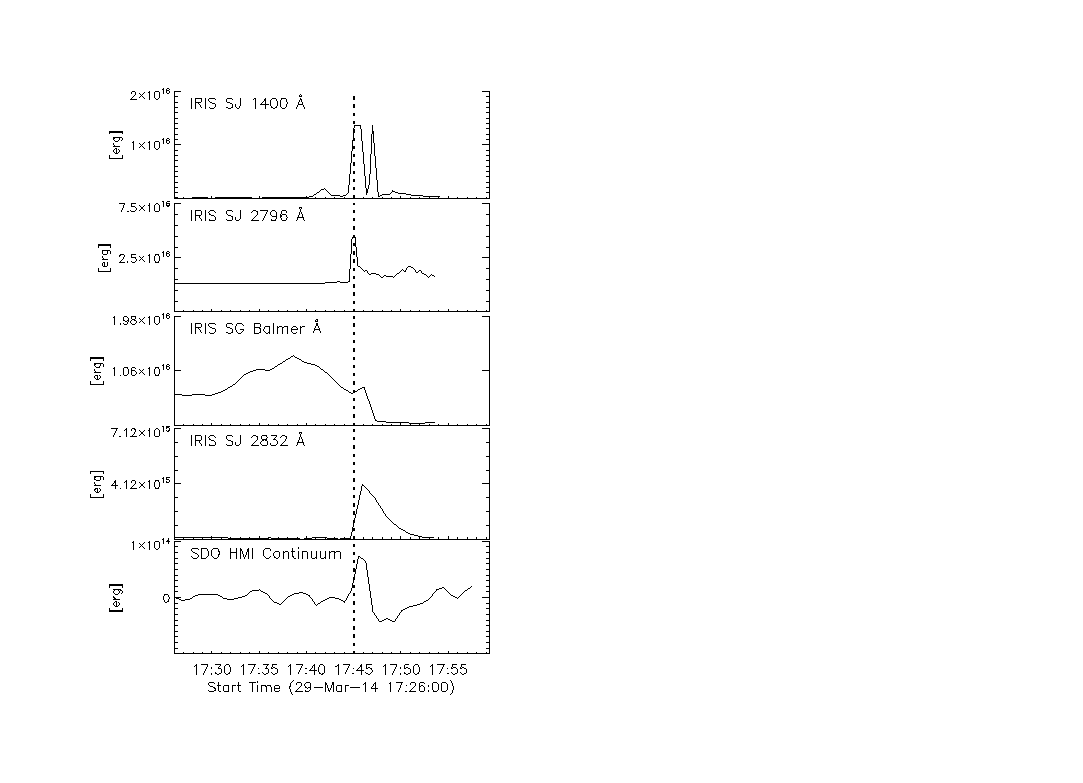
\includegraphics[width=0.6\textwidth]{29-Mar-14-Ribbon-xyPosition-503-265-Frame-1-Energy-Ladder}
  \end{center}
  \caption{Shows calculated energy (erg) values over time (UT) for the heliocentric coordinates (arcsec) contained in the plot title. Each plot represents an independant data set, in order from top to bottom the sets are; IRIS SJ 1400 \AA\ (Si IV); IRIS SJ 2796 \AA\ (Mg II); IRIS SG  2825.7 to 2825.8 \AA\ (Balmer Continuum);IRIS SJ 2832 \AA\ (Mg II wing); SDO HMI continuum (HMI).}\label{erb7}
\end{figure}

\begin{figure}[H]
  \begin{center}
  \textbf{Energy Over Time, Ribbon Location: x = 506, y = 268 }\par\medskip
  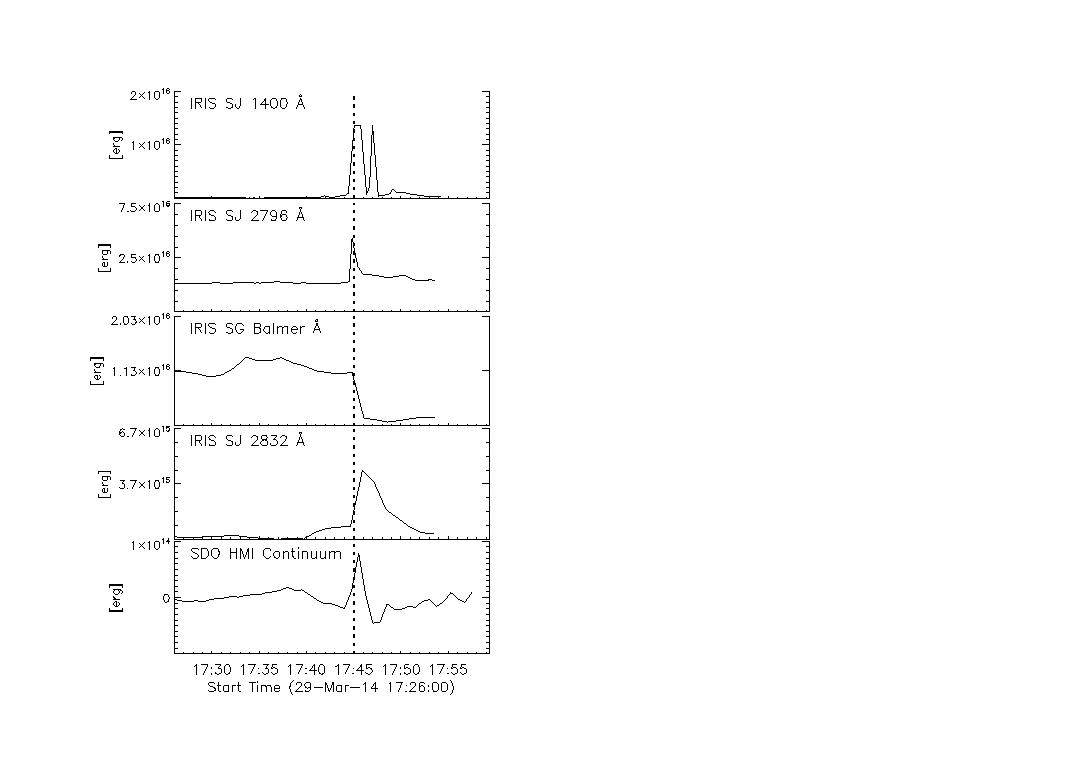
\includegraphics[width=0.6\textwidth]{29-Mar-14-Ribbon-xyPosition-506-268-Frame-1-Energy-Ladder}
  \end{center}
  \caption{Shows calculated energy (erg) values over time (UT) for the heliocentric coordinates (arcsec) contained in the plot title. Each plot represents an independant data set, in order from top to bottom the sets are; IRIS SJ 1400 \AA\ (Si IV); IRIS SJ 2796 \AA\ (Mg II); IRIS SG  2825.7 to 2825.8 \AA\ (Balmer Continuum);IRIS SJ 2832 \AA\ (Mg II wing); SDO HMI continuum (HMI).}\label{erb8}
\end{figure}

\begin{figure}[H]
  \begin{center}
  \textbf{Energy Over Time, Ribbon Location: x = 509, y = 268 }\par\medskip
  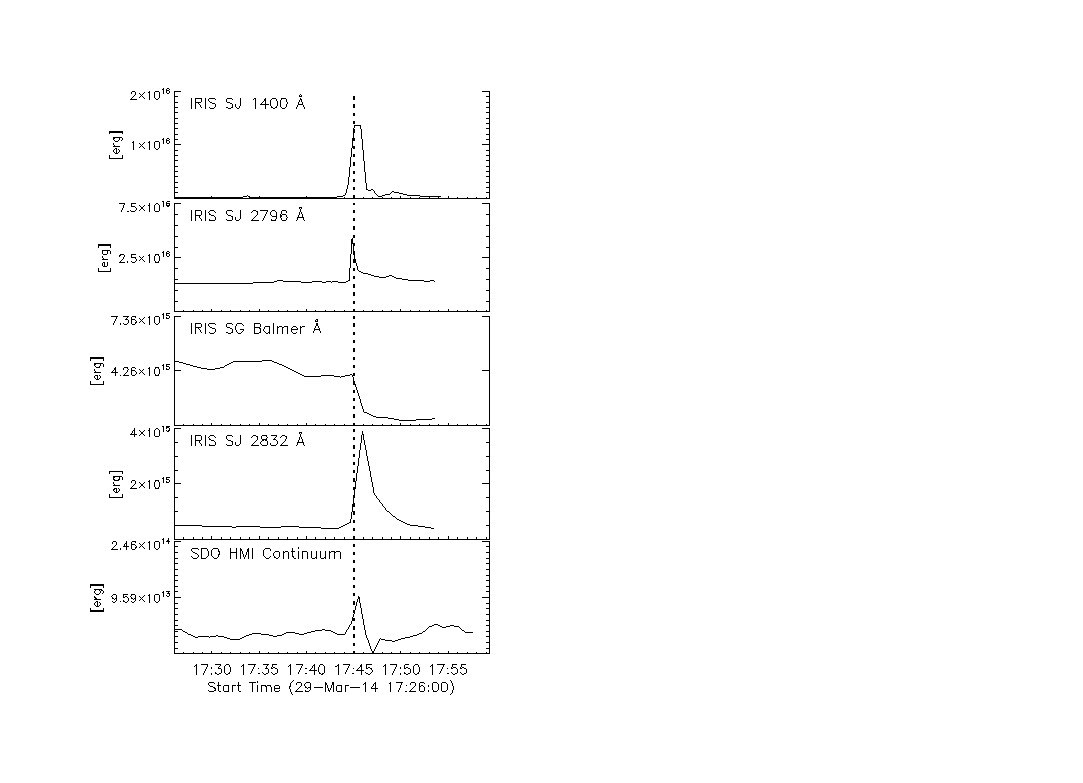
\includegraphics[width=0.6\textwidth]{29-Mar-14-Ribbon-xyPosition-509-268-Frame-1-Energy-Ladder}
  \end{center}
  \caption{Shows calculated energy (erg) values over time (UT) for the heliocentric coordinates (arcsec) contained in the plot title. Each plot represents an independant data set, in order from top to bottom the sets are; IRIS SJ 1400 \AA\ (Si IV); IRIS SJ 2796 \AA\ (Mg II); IRIS SG  2825.7 to 2825.8 \AA\ (Balmer Continuum);IRIS SJ 2832 \AA\ (Mg II wing); SDO HMI continuum (HMI).}\label{erb9}
\end{figure}

\begin{figure}[H]
  \begin{center}
  \textbf{Energy Over Time, Ribbon Location: x = 514, y = 270 }\par\medskip
  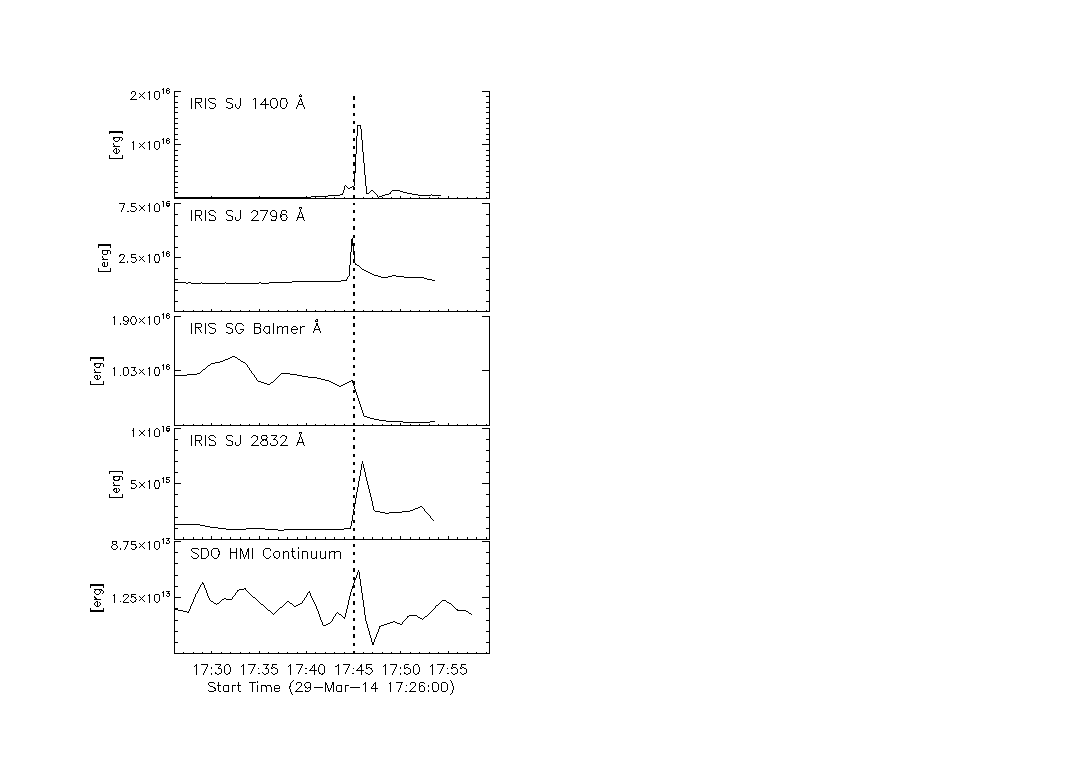
\includegraphics[width=0.6\textwidth]{29-Mar-14-Ribbon-xyPosition-514-270-Frame-1-Energy-Ladder}
  \end{center}
  \caption{Shows calculated energy (erg) values over time (UT) for the heliocentric coordinates (arcsec) contained in the plot title. Each plot represents an independant data set, in order from top to bottom the sets are; IRIS SJ 1400 \AA\ (Si IV); IRIS SJ 2796 \AA\ (Mg II); IRIS SG  2825.7 to 2825.8 \AA\ (Balmer Continuum);IRIS SJ 2832 \AA\ (Mg II wing); SDO HMI continuum (HMI).}\label{erb10}
\end{figure}

\begin{figure}[H]
  \begin{center}
  \textbf{Energy Over Time, Ribbon Location: x = 518, y = 259 }\par\medskip
  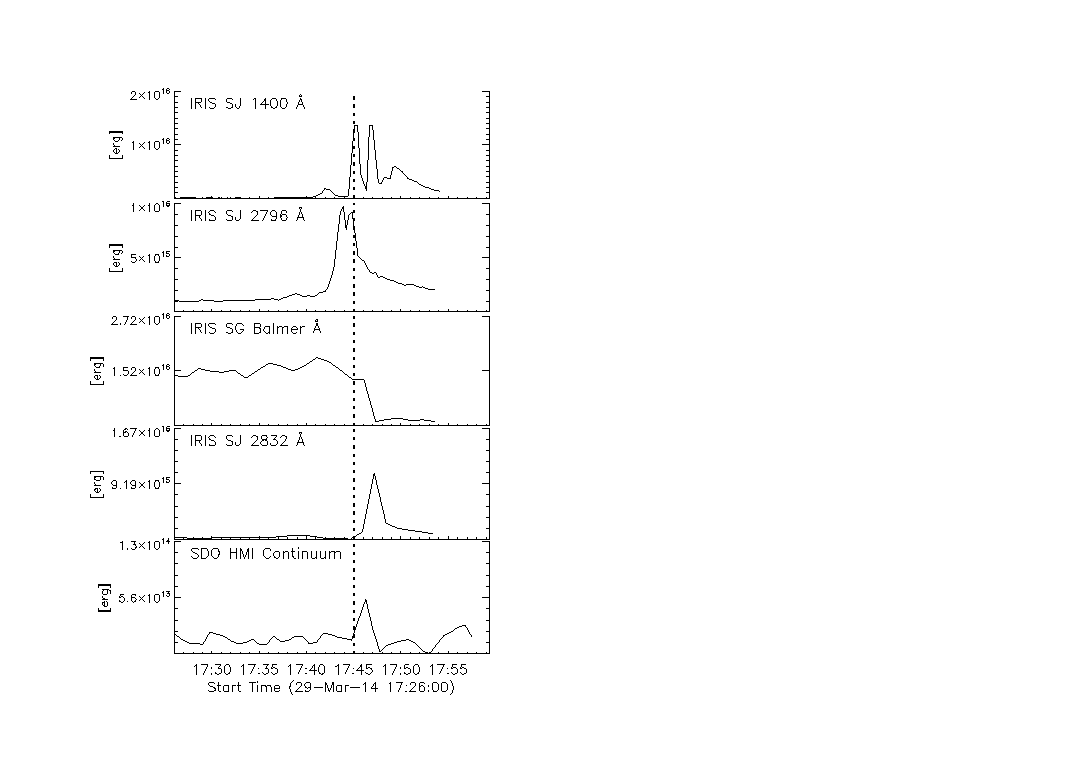
\includegraphics[width=0.6\textwidth]{29-Mar-14-Ribbon-xyPosition-518-259-Frame-2-Energy-Ladder}
  \end{center}
  \caption{Shows calculated energy (erg) values over time (UT) for the heliocentric coordinates (arcsec) contained in the plot title. Each plot represents an independant data set, in order from top to bottom the sets are; IRIS SJ 1400 \AA\ (Si IV); IRIS SJ 2796 \AA\ (Mg II); IRIS SG  2825.7 to 2825.8 \AA\ (Balmer Continuum);IRIS SJ 2832 \AA\ (Mg II wing); SDO HMI continuum (HMI).}\label{erb11}
\end{figure}

\begin{figure}[H]
  \begin{center}
  \textbf{Energy Over Time, Ribbon Location: x = 519, y = 259 }\par\medskip
  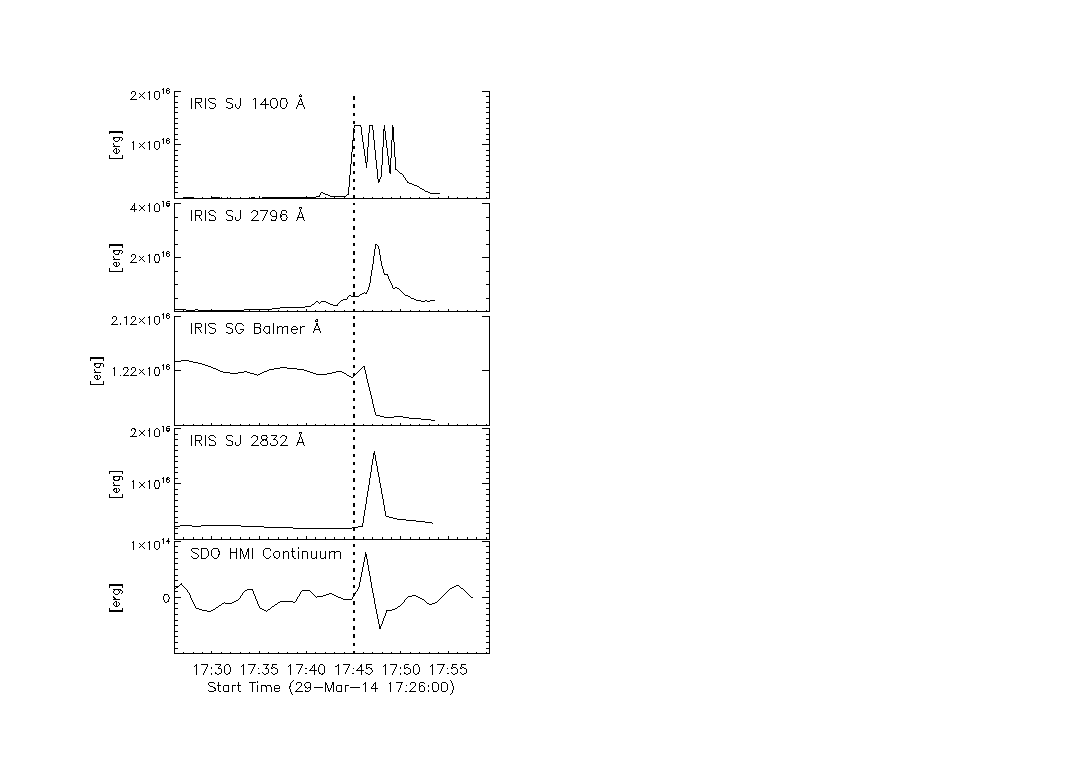
\includegraphics[width=0.6\textwidth]{29-Mar-14-Ribbon-xyPosition-519-259-Frame-2-Energy-Ladder}
  \end{center}
  \caption{Shows calculated energy (erg) values over time (UT) for the heliocentric coordinates (arcsec) contained in the plot title. Each plot represents an independant data set, in order from top to bottom the sets are; IRIS SJ 1400 \AA\ (Si IV); IRIS SJ 2796 \AA\ (Mg II); IRIS SG  2825.7 to 2825.8 \AA\ (Balmer Continuum);IRIS SJ 2832 \AA\ (Mg II wing); SDO HMI continuum (HMI).}\label{erb12}
\end{figure}

\begin{figure}[H]
  \begin{center}
  \textbf{Energy Over Time, Ribbon Location: x = 520, y = 259 }\par\medskip
  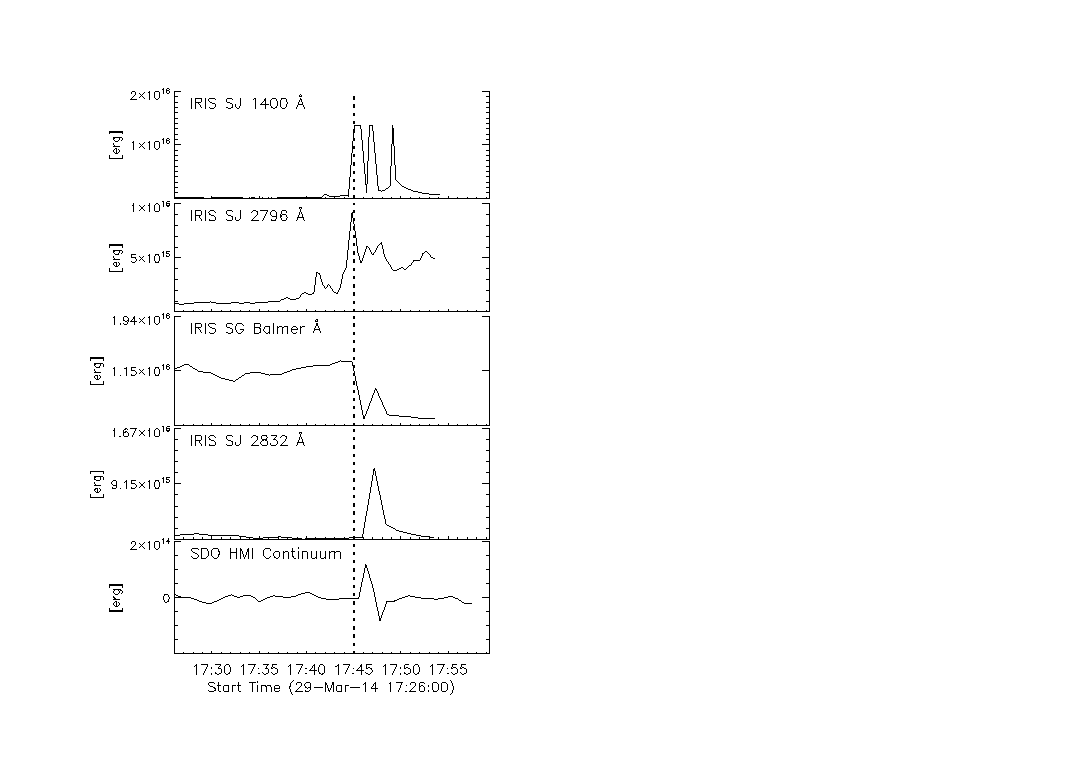
\includegraphics[width=0.6\textwidth]{29-Mar-14-Ribbon-xyPosition-520-259-Frame-2-Energy-Ladder}
  \end{center}
  \caption{Shows calculated energy (erg) values over time (UT) for the heliocentric coordinates (arcsec) contained in the plot title. Each plot represents an independant data set, in order from top to bottom the sets are; IRIS SJ 1400 \AA\ (Si IV); IRIS SJ 2796 \AA\ (Mg II); IRIS SG  2825.7 to 2825.8 \AA\ (Balmer Continuum);IRIS SJ 2832 \AA\ (Mg II wing); SDO HMI continuum (HMI).}\label{erb13}
\end{figure}

\begin{figure}[H]
  \begin{center}
  \textbf{Energy Over Time, Ribbon Location: x = 521, y = 259 }\par\medskip
  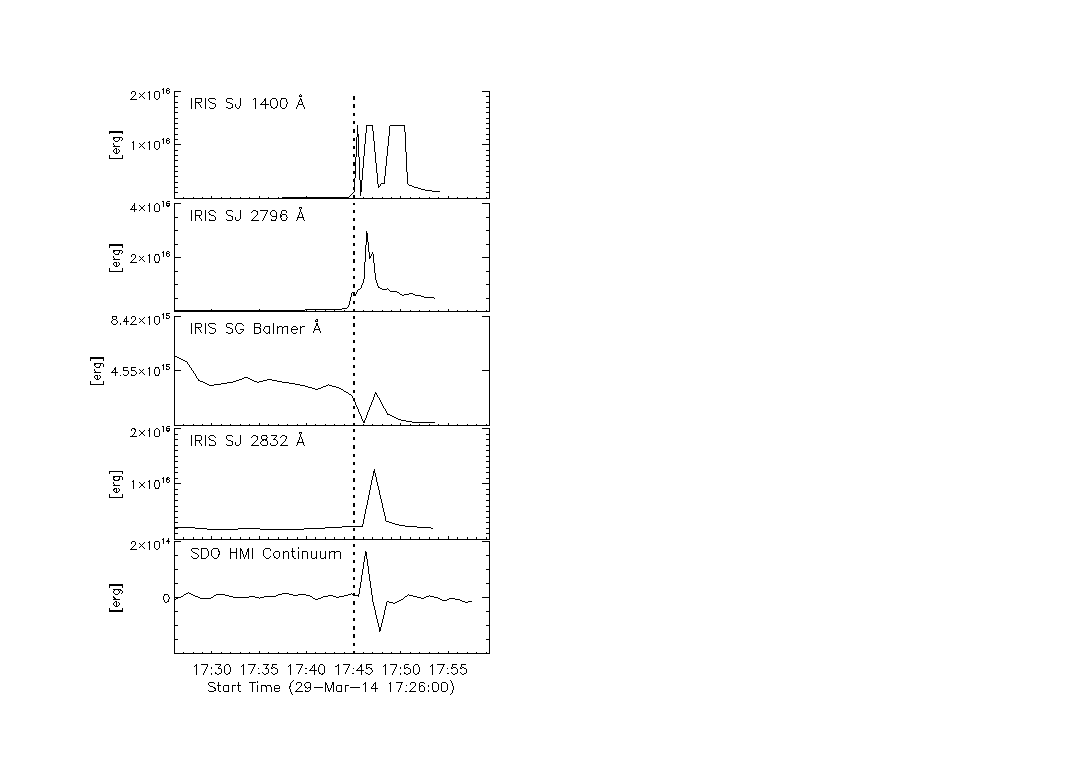
\includegraphics[width=0.6\textwidth]{29-Mar-14-Ribbon-xyPosition-521-259-Frame-2-Energy-Ladder}
  \end{center}
  \caption{Shows calculated energy (erg) values over time (UT) for the heliocentric coordinates (arcsec) contained in the plot title. Each plot represents an independant data set, in order from top to bottom the sets are; IRIS SJ 1400 \AA\ (Si IV); IRIS SJ 2796 \AA\ (Mg II); IRIS SG  2825.7 to 2825.8 \AA\ (Balmer Continuum);IRIS SJ 2832 \AA\ (Mg II wing); SDO HMI continuum (HMI).}\label{erb14}
\end{figure}

\begin{figure}[H]
  \begin{center}
  \textbf{Energy Over Time, Ribbon Location: x = 524, y = 259 }\par\medskip
  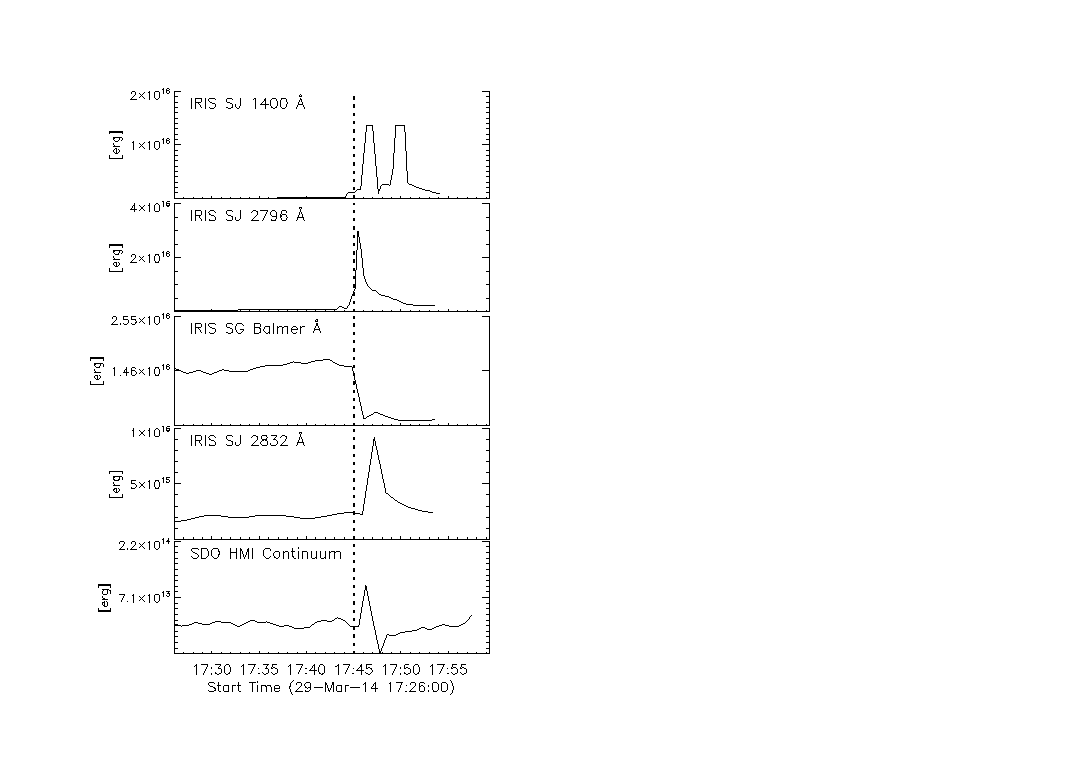
\includegraphics[width=0.6\textwidth]{29-Mar-14-Ribbon-xyPosition-524-259-Frame-2-Energy-Ladder}
  \end{center}
  \caption{Shows calculated energy (erg) values over time (UT) for the heliocentric coordinates (arcsec) contained in the plot title. Each plot represents an independant data set, in order from top to bottom the sets are; IRIS SJ 1400 \AA\ (Si IV); IRIS SJ 2796 \AA\ (Mg II); IRIS SG  2825.7 to 2825.8 \AA\ (Balmer Continuum);IRIS SJ 2832 \AA\ (Mg II wing); SDO HMI continuum (HMI).}\label{erb15}
\end{figure}

\begin{figure}[H]
  \begin{center}
  \textbf{Energy Over Time, Ribbon Location: x = 444, y = 264 }\par\medskip
  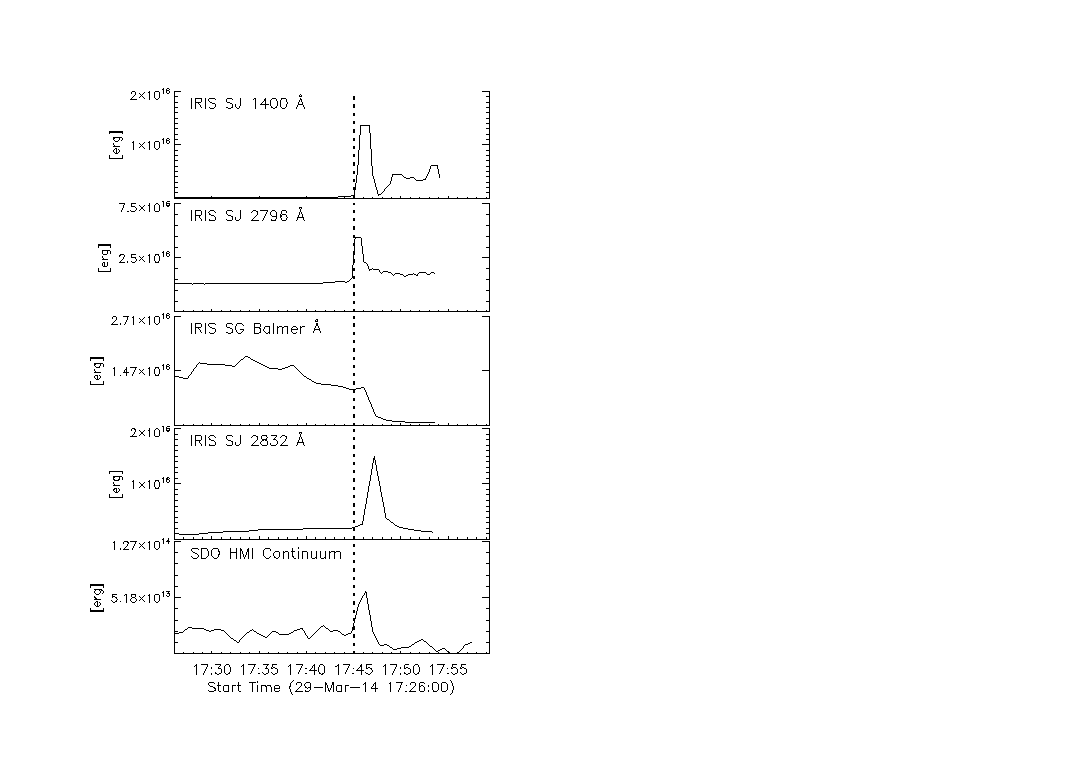
\includegraphics[width=0.6\textwidth]{29-Mar-14-Ribbon-xyPosition-499-264-Frame-2-Energy-Ladder}
  \end{center}
  \caption{Shows calculated energy (erg) values over time (UT) for the heliocentric coordinates (arcsec) contained in the plot title. Each plot represents an independant data set, in order from top to bottom the sets are; IRIS SJ 1400 \AA\ (Si IV); IRIS SJ 2796 \AA\ (Mg II); IRIS SG  2825.7 to 2825.8 \AA\ (Balmer Continuum);IRIS SJ 2832 \AA\ (Mg II wing); SDO HMI continuum (HMI).}\label{erb16}
\end{figure}

\begin{figure}[H]
  \begin{center}
  \textbf{Energy Over Time, Ribbon Location: x = 502, y = 263 }\par\medskip
  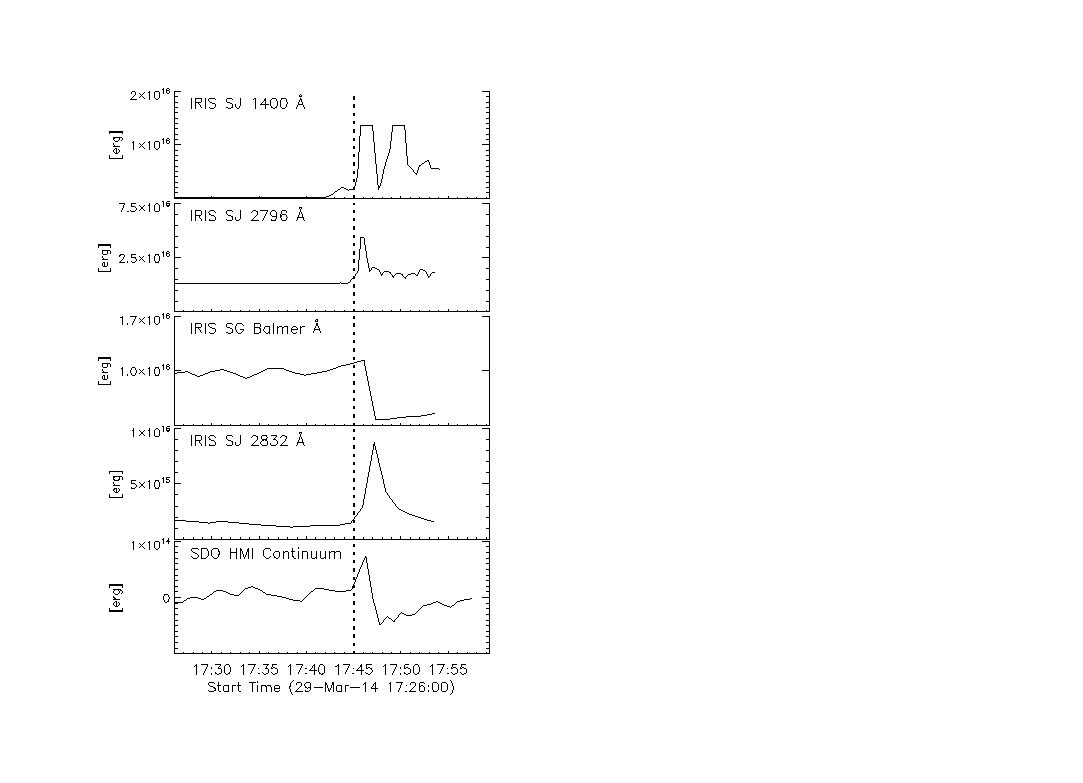
\includegraphics[width=0.6\textwidth]{29-Mar-14-Ribbon-xyPosition-502-263-Frame-2-Energy-Ladder}
  \end{center}
  \caption{Shows calculated energy (erg) values over time (UT) for the heliocentric coordinates (arcsec) contained in the plot title. Each plot represents an independant data set, in order from top to bottom the sets are; IRIS SJ 1400 \AA\ (Si IV); IRIS SJ 2796 \AA\ (Mg II); IRIS SG  2825.7 to 2825.8 \AA\ (Balmer Continuum);IRIS SJ 2832 \AA\ (Mg II wing); SDO HMI continuum (HMI).}\label{erb17}
\end{figure}

\begin{figure}[H]
  \begin{center}
  \textbf{Energy Over Time, Ribbon Location: x = 504, y = 267 }\par\medskip
  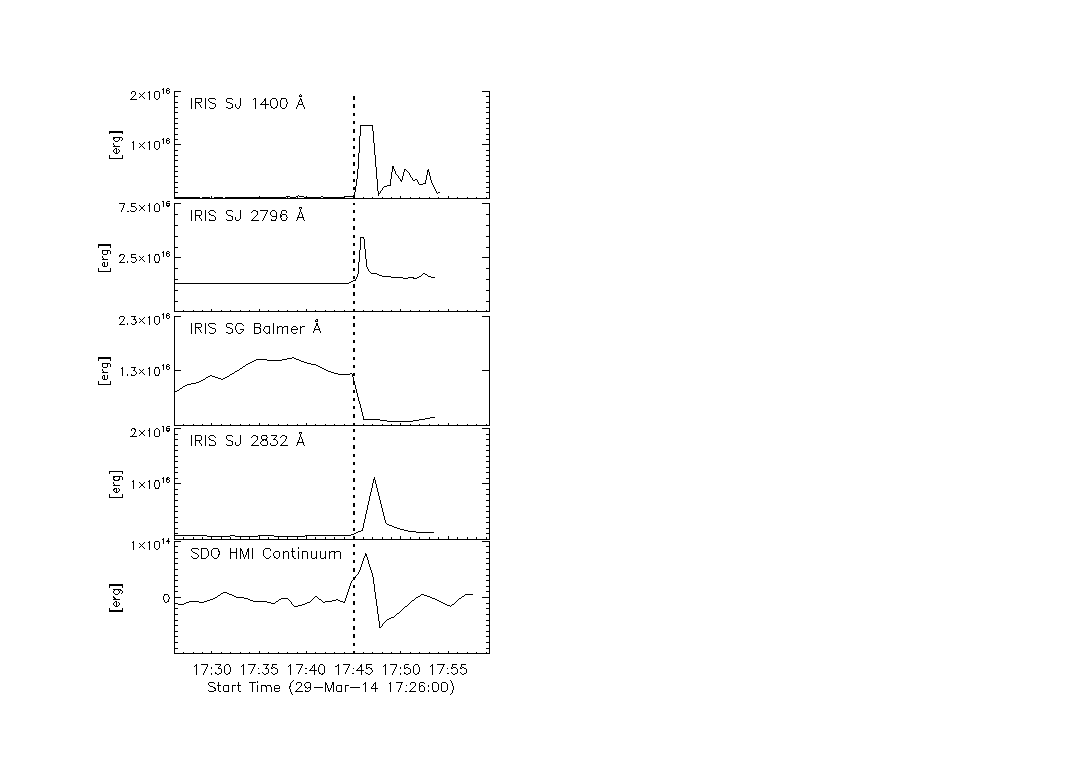
\includegraphics[width=0.6\textwidth]{29-Mar-14-Ribbon-xyPosition-504-267-Frame-2-Energy-Ladder}
  \end{center}
  \caption{Shows calculated energy (erg) values over time (UT) for the heliocentric coordinates (arcsec) contained in the plot title. Each plot represents an independant data set, in order from top to bottom the sets are; IRIS SJ 1400 \AA\ (Si IV); IRIS SJ 2796 \AA\ (Mg II); IRIS SG  2825.7 to 2825.8 \AA\ (Balmer Continuum);IRIS SJ 2832 \AA\ (Mg II wing); SDO HMI continuum (HMI).}\label{erb18}
\end{figure}

\begin{figure}[H]
  \begin{center}
  \textbf{Energy Over Time, Ribbon Location: x = 508, y = 269 }\par\medskip
  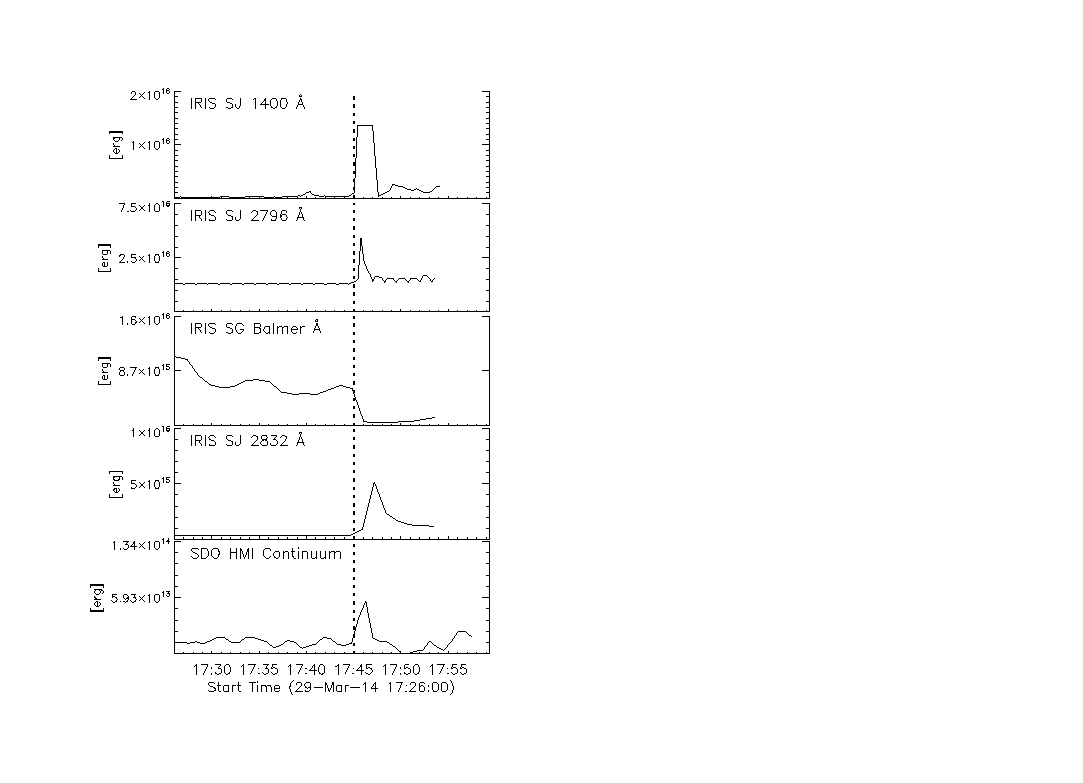
\includegraphics[width=0.6\textwidth]{29-Mar-14-Ribbon-xyPosition-508-269-Frame-2-Energy-Ladder}
  \end{center}
  \caption{Shows calculated energy (erg) values over time (UT) for the heliocentric coordinates (arcsec) contained in the plot title. Each plot represents an independant data set, in order from top to bottom the sets are; IRIS SJ 1400 \AA\ (Si IV); IRIS SJ 2796 \AA\ (Mg II); IRIS SG  2825.7 to 2825.8 \AA\ (Balmer Continuum);IRIS SJ 2832 \AA\ (Mg II wing); SDO HMI continuum (HMI).}\label{erb19}
\end{figure}

\begin{figure}[H]
  \begin{center}
  \textbf{Energy Over Time, Ribbon Location: x = 511, y = 272 }\par\medskip
  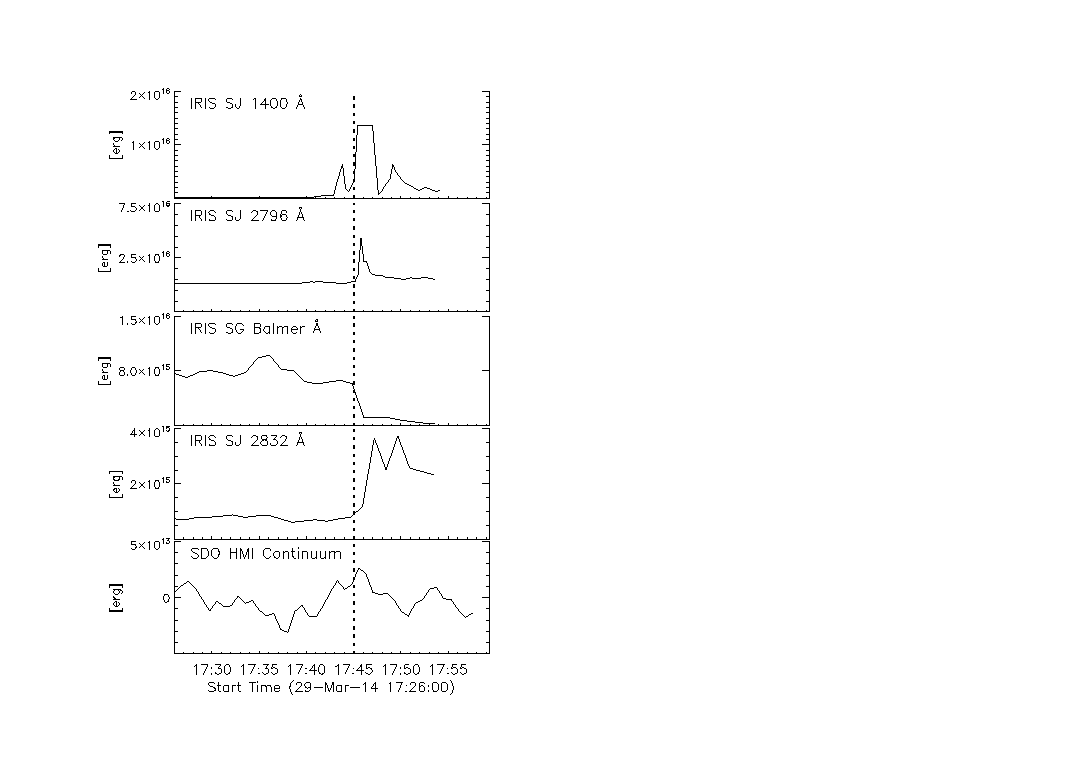
\includegraphics[width=0.6\textwidth]{29-Mar-14-Ribbon-xyPosition-511-272-Frame-2-Energy-Ladder}
  \end{center}
  \caption{Shows calculated energy (erg) values over time (UT) for the heliocentric coordinates (arcsec) contained in the plot title. Each plot represents an independant data set, in order from top to bottom the sets are; IRIS SJ 1400 \AA\ (Si IV); IRIS SJ 2796 \AA\ (Mg II); IRIS SG  2825.7 to 2825.8 \AA\ (Balmer Continuum);IRIS SJ 2832 \AA\ (Mg II wing); SDO HMI continuum (HMI).}\label{erb20}
\end{figure}












% \begin{table}%[H]
% \centering
% \begin{tabular}{|c|c|c|c|c|c|c|c|}
% Time UT & Sunquake Coords x",y"  & $E_{Si IV}$ & $E_{Mg II}$ & $E_{Balm}$ & $E_{Mg II w}$ & $E_{HMI}$ & $E_{area}$\\
% \hline
% 17:45 & 518.5, 264.0 & 9.63E+14 & 4.36E+16 & 2.68E+16 & 3.29E+13 & 8.21E+15 & 7.26E+15\\
% 17:46 & 518.5, 264.0 & 2.52E+15 & 1.58E+16 & 5.00E+15 & -4.48E+12 & 5.31E+15 & -1.12E+15\\
% \end{tabular}
% \caption{Pixel coordinates in arcsecs and Energies in ergs at 17:45 and 17:46 for the sunquake pixel and area. *coordinates are the central pixel of a 13 pixel sunquake area}\label{qkenergytab}
% \end{table}
\begin{table}[H]
\centering
\begin{tabular}{|c|c|c|c|c|c|c|c|}
Time UT & Sunquake Coords x",y"  & $E_{Si IV}$ & $E_{Mg II}$ & $E_{Balm}$ & $E_{Mg II w}$ & $E_{HMI}$ & $E_{area}$\\
\hline
17:45 & 518.5, 264.0 & 9.63E+14 & 4.36E+16 & 2.68E+16 & 8.21E+15 & 3.29E+13 & 2.54E+17\\
17:46 & 518.5, 264.0 & 2.52E+15 & 1.58E+16 & 5.00E+15 & 5.31E+15 & 3.18E+13 & 2.51E+17\\
\end{tabular}
\caption{Pixel coordinates in arcsecs and Energies in ergs at 17:45 and 17:46 for the sunquake pixel and area. *coordinates are the central pixel of a 13 pixel sunquake area}\label{qkenergytab}
\end{table}


\begin{sidewaystable}[h]
\tiny
\centering
\begin{tabular}{|c|c|c|c|c|c|c|c|c|c|c|}
Time & Si Coords (x,y) & $E_{Si IV}$ & Mg Coords(x,y) & $E_{Mg II}$ & Balm Coords(x,y) & $E_{Balm}$ & Mgw Coords (x,y) & $E_{Mg II w}$ & HMI Coords (x,y) & $E_{HMI}$\\
\hline
17:45 & 517.54, 261.58 & 1.78E+15 & 496.03, 263.76 & 2.34E+16 & 517.80, 260.50 & 1.26E+16 & 517.14, 261.79 & 9.32E+15 & 517.80, 260.50 & 5.83E+13\\
17:45 & 517.54, 264.13 & 5.93E+14 & 502.50, 264.93 & 1.58E+16 & 518.80, 261.00 & 1.97E+16 & 518.68, 262.86 & 8.47E+15 & 518.80, 261.00 & 1.15E+14\\
17:45 & 518.02, 266.35 & 1.37E+16 & 504.66, 268.10 & 4.36E+16 & 519.70, 261.70 & 8.93E+15 & 519.61, 263.79 & 2.29E+16 & 519.70, 261.70 & 1.64E+14\\
17:45 & 519.29, 267.78 & 1.37E+16 & 509.13, 269.64 & 1.58E+16 & 520.60, 262.30 & 7.01E+15 & 521.15, 264.87 & 7.76E+15 & 520.60, 262.30 & 1.48E+14\\
17:45 & 522.31, 267.14 & 1.37E+16 & 514.09, 271.49 & 4.36E+16 & 521.70, 262.60 & 5.51E+15 & 523.46, 265.18 & 8.83E+15 & 521.70, 262.60 & 1.17E+14\\
17:45 & 496.03, 264.56 & 2.69E+15 & 517.48, 262.95 & 4.36E+16 & 500.70, 262.70 & 1.12E+16 & 496.03, 264.56 & 5.77E+15 & 500.70, 262.70 & 6.66E+13\\
17:45 & 502.20, 265.18 & 1.37E+16 & 518.60, 264.07 & 4.36E+16 & 503.80, 265.00 & 7.97E+15 & 502.20, 265.18 & 4.10E+15 & 503.80, 265.00 & 7.39E+13\\
17:45 & 504.66, 268.10 & 1.37E+16 & 519.44, 265.75 & 4.36E+16 & 506.90, 268.10 & 3.48E+15 & 504.66, 268.10 & 4.43E+15 & 506.90, 268.10 & 7.90E+13\\
17:45 & 509.13, 269.64 & 1.37E+16 & 520.55, 266.86 & 4.36E+16 & 509.28, 268.79 & 1.94E+15 & 509.13, 269.64 & 3.90E+15 & 509.28, 268.79 & 1.00E+14\\
17:45 & 513.29, 271.65 & 2.37E+15 & 524.47, 265.47 & 4.36E+16 & 514.40, 270.10 & 3.17E+15 & 513.29, 271.65 & 7.01E+15 & 514.40, 270.10 & 4.93E+13\\
17:46 & 499.88, 264.87 & 1.39E+15 & 486.52, 264.28 & 4.85E+15 & 518.60, 259.10 & 4.08E+15 & 517.91, 260.40 & 1.07E+16 & 518.60, 259.10 & 5.33E+13\\
17:46 & 502.35, 266.56 & 5.73E+15 & 497.24, 265.62 & 6.50E+15 & 519.60, 259.30 & 5.03E+15 & 519.76, 259.94 & 1.60E+16 & 519.60, 259.30 & 7.99E+13\\
17:46 & 503.89, 268.57 & 1.06E+15 & 500.22, 267.63 & 4.48E+15 & 520.60, 259.50 & 9.00E+15 & 521.77, 259.47 & 1.14E+16 & 520.60, 259.50 & 1.20E+14\\
17:46 & 506.97, 270.72 & 1.37E+16 & 505.29, 269.47 & 8.83E+15 & 521.60, 259.90 & 3.02E+15 & 523.77, 258.86 & 1.26E+16 & 521.60, 259.90 & 1.67E+14\\
17:46 & 511.29, 272.11 & 1.37E+16 & 512.73, 271.15 & 2.33E+16 & 524.10, 259.70 & 6.31E+15 & 524.69, 260.24 & 9.22E+15 & 524.10, 259.70 & 1.04E+14\\
17:46 & 515.18, 261.86 & 1.37E+16 & 517.98, 261.31 & 4.36E+16 & 499.10, 264.70 & 4.50E+15 & 499.88, 264.87 & 1.51E+16 & 499.10, 264.70 & 6.05E+13\\
17:46 & 517.70, 261.58 & 1.37E+16 & 519.09, 261.31 & 4.36E+16 & 502.10, 263.80 & 3.60E+15 & 502.35, 266.56 & 8.74E+15 & 502.10, 263.80 & 7.39E+13\\
17:46 & 520.21, 262.41 & 1.37E+16 & 521.33, 261.31 & 4.36E+16 & 504.60, 267.00 & 3.95E+15 & 503.89, 268.57 & 1.12E+16 & 504.60, 267.00 & 7.88E+13\\
17:46 & 523.28, 262.97 & 1.37E+16 & 522.73, 261.31 & 4.36E+16 & 508.40, 269.80 & 2.03E+15 & 506.97, 270.72 & 5.20E+15 & 508.40, 269.80 & 5.43E+13\\
17:46 & 525.52, 263.81 & 1.37E+16 & 524.68, 262.99 & 4.36E+16 & 511.00, 272.00 & 1.95E+15 & 511.29, 272.11 & 3.66E+15 & 511.00, 272.00 & 2.14E+13\\
\end{tabular}
\caption{Coordinates and Energies at 17:45 and 17:46 for ribbon sample locations.}\label{ribenergytab}
\end{sidewaystable}
